Para medir las longitudes de onda de las líneas del espectro de Hidrógeno, se 
utilizó un espectrogoniómetro para medir los ángulos de difracción de tres 
líneas del espectro.

Para realizar las mediciones correctamente, es necesario calibrar el 
espectrogoniómetro. Para ello, se colocó frente a la lámpara de hidrógeno, 
alineando el tubo del colimador de manera que coincidiera con la luz emitida 
por la lámpara. Luego, el tubo del ocular se ajustó al tubo del colimador hasta 
que el haz de luz fuera claramente visible a través del ocular. Una vez que 
ambos tubos estuvieron correctamente alineados, se movió el disco de Vernier 
hasta que los ceros coincidieran.

Con el espectrogoniómetro calibrado, se colocó la rejilla de difracción de 600 
divisiones por milímetro. Este montaje se muestra en la 
\cref{fig:experimental-setup-H}.

\begin{figure}[htbp!]
  \begin{center}
    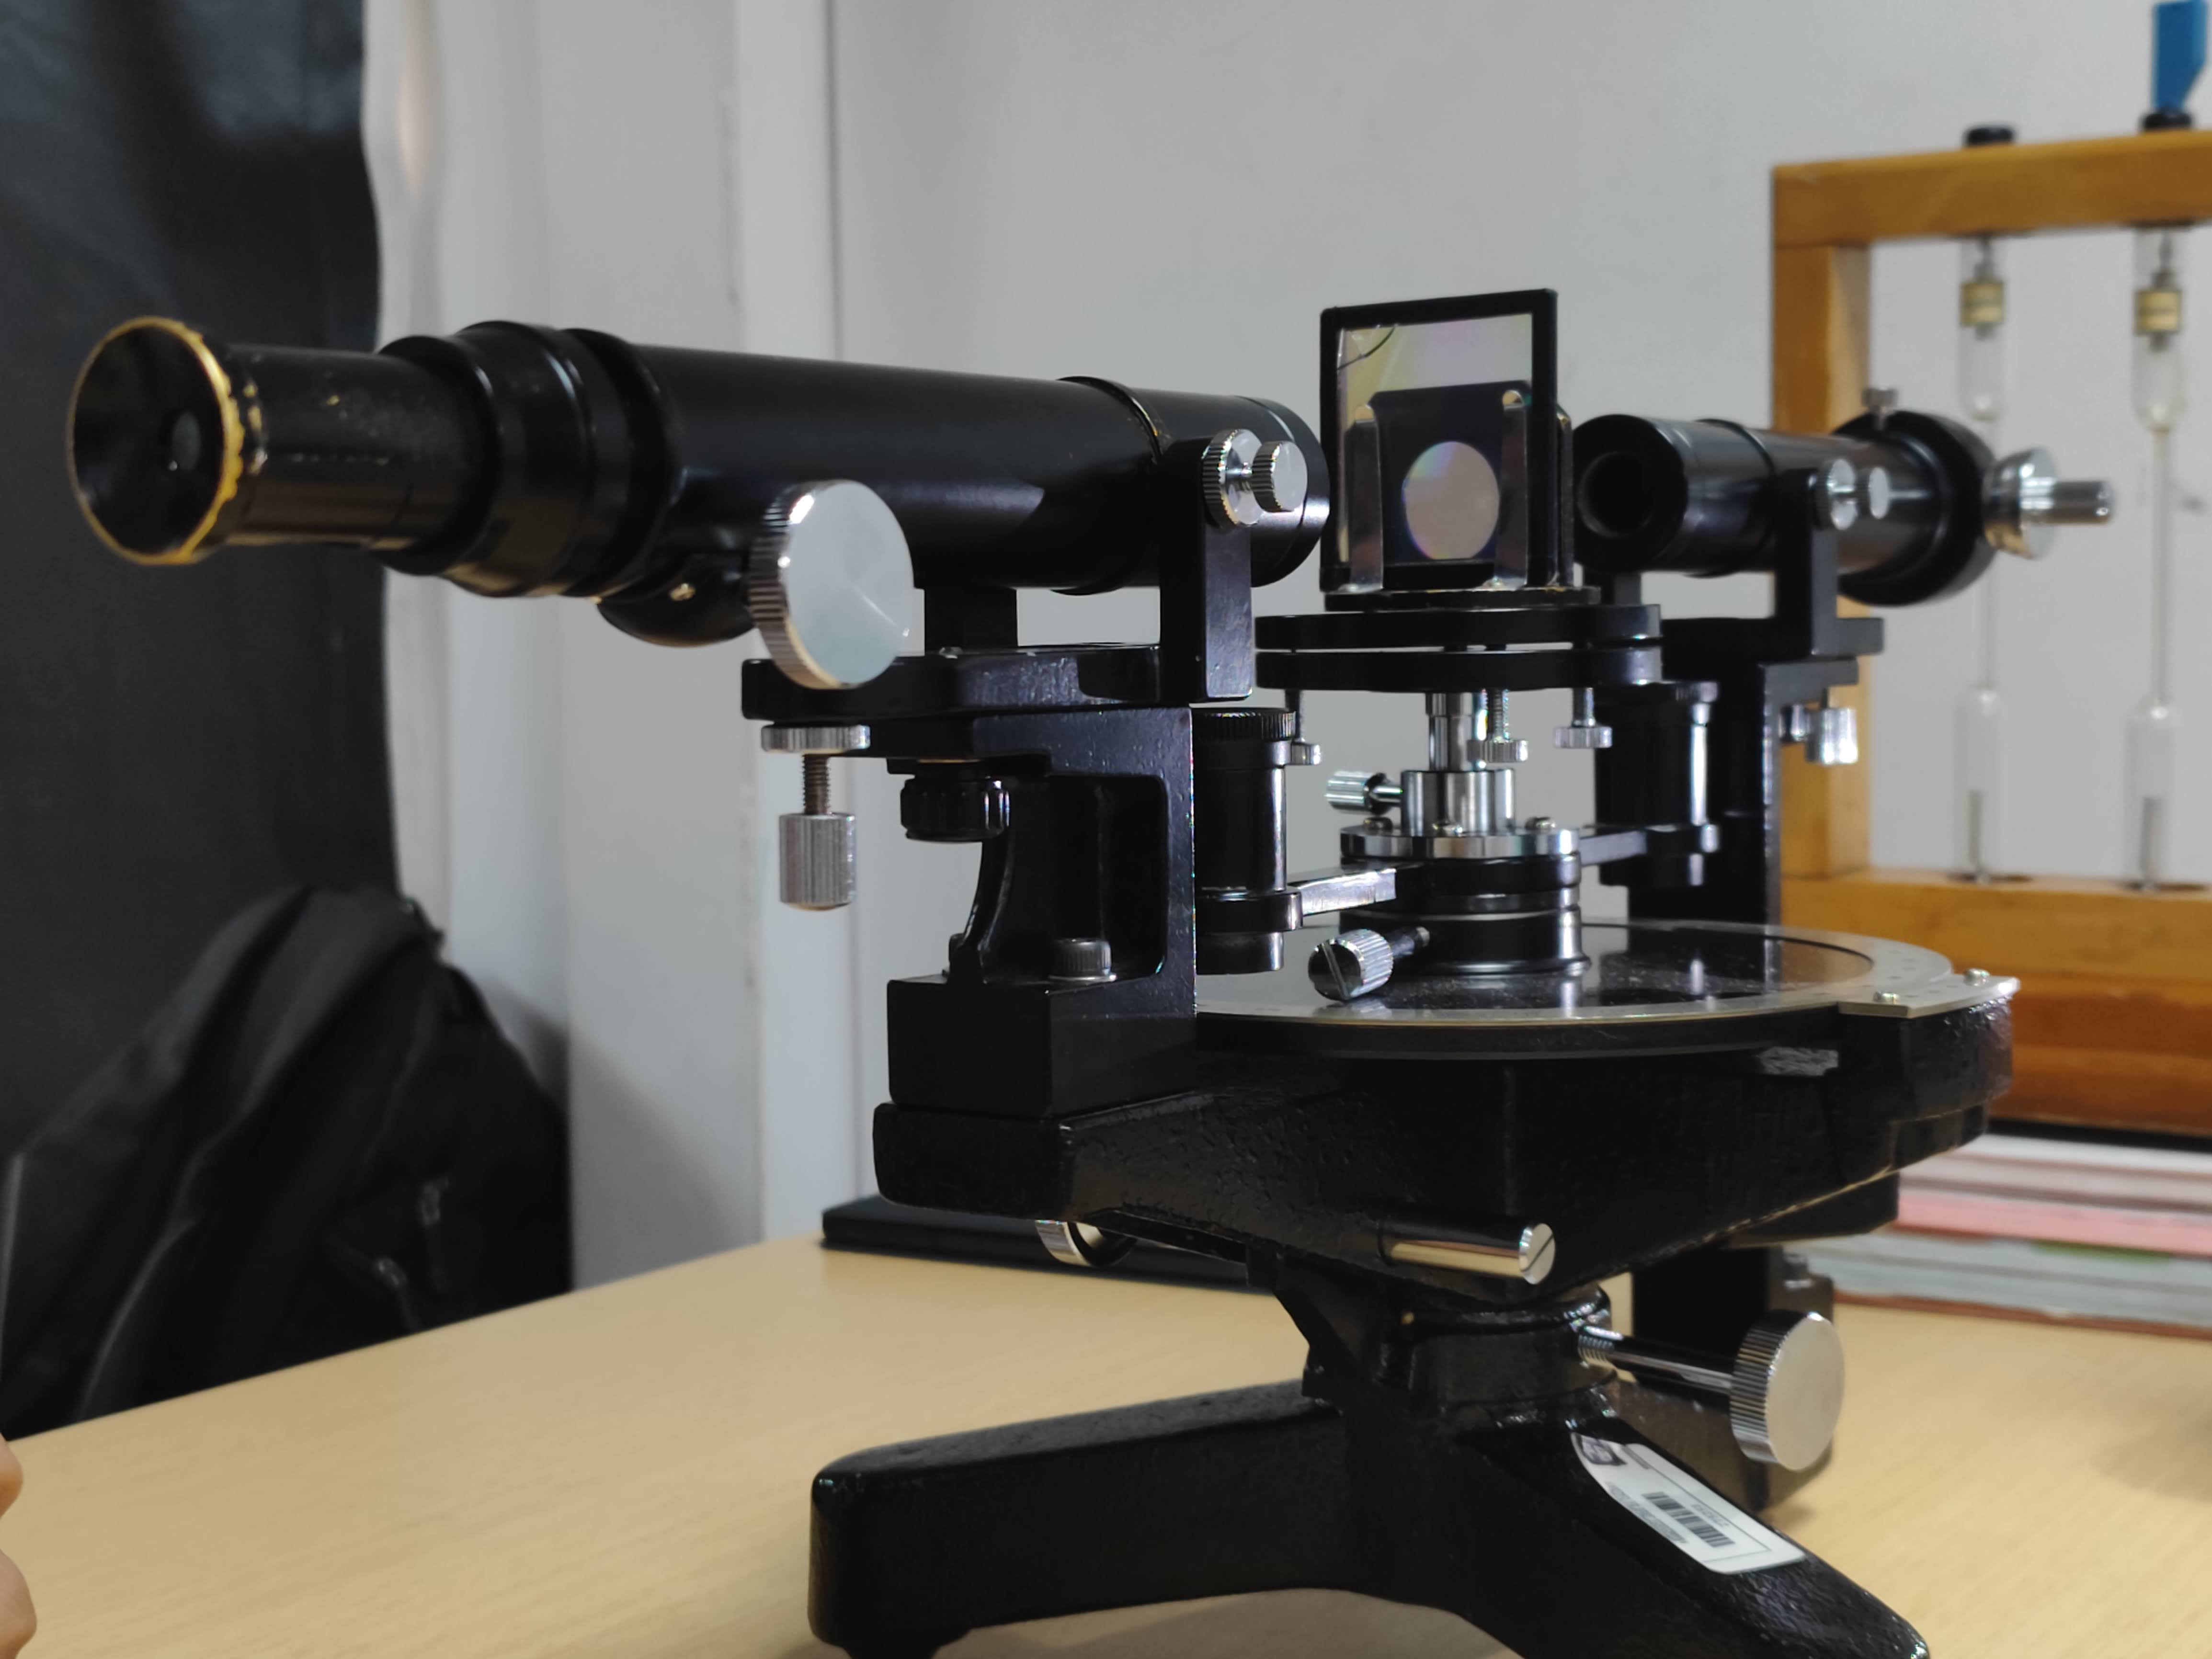
\includegraphics[width=\linewidth]{./Figures/experimental-setup-H.jpg}
    \caption{Montaje experimental para el Hidrógeno.}
    \label{fig:experimental-setup-H}
	\end{center}
\end{figure}

Para medir los ángulos, el tubo del ocular se movió hasta centrar la línea roja 
del espectro en el ocular. El ángulo de esta línea espectral se determinó 
ubicando primero el cero del disco de Vernier, que indica el valor del ángulo.

Una vez calculado el ángulo de la línea roja, se repitió el mismo procedimiento 
para las líneas espectrales de color cian y azul.

Para el caso del elemento desconocido, se siguió el mismo procedimiento que 
para el hidrógeno, midiendo los ángulos correspondientes a las líneas 
espectrales entre los colores rojo, naranja y amarillo. El montaje experimental 
utilizado se muestra en la \cref{fig:experimental-setup-Na}.

\begin{figure}[htbp!]                                                           
  \begin{center}                                                              
    \includegraphics[height=0.9\linewidth, page=2]{./Figures/experimental-setup-Na.jpg}
    \caption{Montaje experimental para el elemento desconocido.}                         
    \label{fig:experimental-setup-Na}                                          
  \end{correctamenter}                                                                
\end{figure}
